  \item Zwolnienie pracownika \\
  
  Opis słowny - współpraca z pracownikiem kiedyś dobiega końca, w takiej
  sytuacji uprawniona osoba musi usunąć takiego pracownika z systemu poprzez
  opcję zwolnienia. Informacje o tej osobie nie są usuwane bezpowrotnie lecz
  archiwizowane zgodnie z przepisami aktualnego prawa.
  
  \begin{longtable}{|p{5cm}|p{7cm}|}
 	\hline
	\textbf{Aktor} & Kierownik \\
	\hline
	\textbf{Warunki początkowe} & Kierwonik zalogowany	\\
	\hline
	\textbf{Opis przebiegu interakcji} & Wyświetlenie listy pracowników,
	zaznaczenia konkretnej osoby, wybór opcji zwolnienia \\
	\hline
	\textbf{Sytuacje wyjątkowe} & Brak \\
	\hline
	\textbf{Warunki końcowe} & Wybrany pracownik nie pojawia się więcej na liście
	pracowników, jego dane są zarchiwizowane. 	\\
	\hline
 \end{longtable}
  
  \begin{tabularx}{\linewidth}{ c X }
  Aktor: & Kierownik \\
  \end{tabularx}
   \begin{enumerate}
    \item Kierownik uruchamia stronę internetową panelu zarządzania sklepem i~wybiera panel zarządzania pracownikami.
    \item Kierownik wyszukuje odpowiedniego pracownika.
    \item System wyświetla pracowników spełniających zadane kryteria wyszukiwania.
    \item Kierownik wybiera odpowiedniego pracownika.
    \item Kierownik wybiera opcję ,,Zwolnij''.
    \item System wyświetla formularz zwolnienia.
    \item Kierownik wypełnia formualrz podając przyczynę zwolnienia oraz datę od której pracownik ma być zwolniony.
    \item System sprawdza poprawność formualrza (np. czy można zwolnić pracownika w terminie wskazanym przez kierownika).
    \item W przypadku błędów system wyświetla odpowiedni komunikat, a kierownik poprawia dane w formularzu.
    \item System wyświetla prośbę o potwierdzenie operacji (dane pracownika oraz pytanie czy na pewno intencją kierownika
    było jego zwolnienie).
    \item Pracownik zatwierdza operację.
    \item System zapisuje informację o zwolnieniu pracownika.
    \item W momencie zaczęcia obowiązywania zwolnienia, system archiwizuje dane pracownika i~usuwa
    go~z~grupy zatrudnionych osób.
  \end{enumerate}

  \begin{figure}[H]
    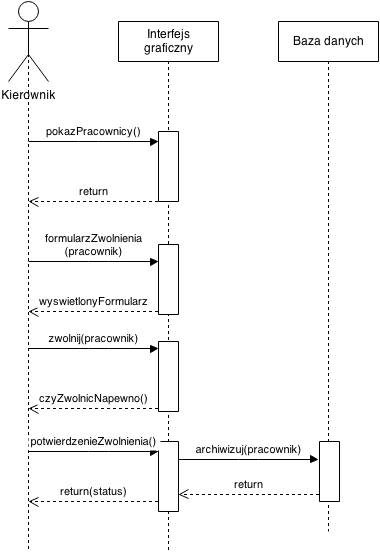
\includegraphics[width=\textwidth,
    height=0.5\textheight]{graphics/UseCase/Pracownik/ZwolnieniePracownika.png}
  \caption{Diagram sekwencji dla przypadku użycia Zwolnienie pracownika -
  scenariusz główny}
\end{figure}